\documentclass[conference]{IEEEtran}
% \IEEEoverridecommandlockouts
% The preceding line is only needed to identify funding in the first footnote. If that is unneeded, please comment it out.
\usepackage{cite}
\usepackage{amsmath,amssymb,amsfonts}
\usepackage{algorithmic}
\usepackage{graphicx}
\usepackage{booktabs}
\usepackage{textcomp}
\usepackage{xcolor}
\usepackage{float}
\def\BibTeX{{\rm B\kern-.05em{\sc i\kern-.025em b}\kern-.08em
    T\kern-.1667em\lower.7ex\hbox{E}\kern-.125emX}}

\begin{document}

\title{PPOrphIt: PPO Robot Manipulator Morphology Design}

\author{\IEEEauthorblockN{Steve Gillet}
\IEEEauthorblockA{\textit{University of Colorado Boulder Robotics} \\
\textit{Email: steve.gillet@colorado.edu}}
% Add more authors if team members are known, e.g.:
\and
\IEEEauthorblockN{Jay Vakil}
\IEEEauthorblockA{\textit{Email: Jay.Vakil@colorado.edu}}
% \and
% \IEEEauthorblockN{Team Member 3}
% \IEEEauthorblockA{\textit{Email: member3.email@example.com}}
}

\maketitle

\begin{abstract}
This paper aims to address the cost and overactuation of robotics used in manufacturing by leveraging reinforcement learning (RL) to optimize robot morphologies to specific use cases.
RL is the right tool for this job because it can optimize over the large search space of possible robot morphologies and effectively explore large varieties of embodiments.
The core methodology involves using a PPO model to iterate on the different morphologies and MuJoCo to evaluate their effectiveness in simulation.
The evaluation signals will be success, path and energy efficiency, simplicity and manipulability index and these will be used to show the effectiveness of the PPO model at creating morphologies that are faster, more effective, and more efficient for particular tasks.
\end{abstract}

\begin{IEEEkeywords}
reinforcement learning, robot morphology, manipulator design
\end{IEEEkeywords}

\section{Introduction and Motivation}
High costs, lack of tailorability, and lack of retrofitting are some of the most cited problems for the adoption of the robotics in industrial settings \cite{mckinsey2019industrial}.
The most commonly used robotic manipulator in manufacturing is FANUC series of 6-DOF manipulators which cost from \$17,500 to \$400,000 depending on their capacity and customizations \cite{standardbots2025fanucprice}\cite{patentpc2025toprobotics}.
Meanwhile \cite{russo2021task} and \cite{he2019underactuated} show that most manipulators are overactuated, less cost-efficient, and less effective for most tasks they are used in.
We want to address this problem by creating an automation pipeline where you feed in a use case and you get out a robot specifically optimized for that use case.
By matching the robot to the task we can ensure that each robot can perform its task effectively and only the parts needed for that task are used, reducing cost and increasing efficiency.
Here we describe the process by which robot manipulator morphologies are optimized to particular tasks using a PPO agent.

We chose reinforcement learning because morphology design is an optimization problem over a complex, high-dimensional search space and RL can explore and learn optimal designs through trial-and-error in simulation \cite{sutton1988learning}.
We chose PPO because it is robust and on-policy and excels in continuous action spaces which is ideal for morphology design where there are continuous parameters like link lengths \cite{schulman2017proximal}.
This is more effective than imitation learning because imitation learning can only use morphologies that already exist severely limiting sample space and innovation \cite{delgado2022robotics}.
Supervised learning suffers from a very similar issue where labelled data would have to be provided which would be infeasible and there is no mechanism for exploration \cite{kober2013reinforcement}.

The core method is to use stable\_baselines3 PPO implementation to iterate on the design parameters (number of links, joint types (X, Y, Z hinge, and Z actuation), and link lengths), use MuJoCo to simulate that iteration on a simple task using RRTConnect and damped least squares (DLS) inverse kinematics (IK) for the path planning, feed the results (success, efficiency, and manipulability index) back into the PPO model.
We chose RRTConnect because it is simple and has been shown to be faster than other methods \cite{844730} which enables faster and more robust evaluation steps.
We also chose DLS IK for a similar reason, it has been shown to be robust especially in situations where the target position is out of reach \cite{buss2004introduction} which is inevitable in a situation where an agent is exploring morphologies.

The evaluation signals will be successful path planning, path length, energy cost, and manipulability index.
The manipulability index is a measure of a manipulators ability to arbitrarily change the position and orientation of the end effector at a particular point, borrowed from \cite{yoshikawa1985manipulability}.
The hope is that the better morphologies will be able to do the tasks more successfully, efficiently, and quickly while still maintaing some robustness and then we can vary the tasks slightly to find better morphologies for particular tasks.
The tasks will be kept simple but varied in ways to test different types of movements like moving near the base, moving from near to far, different elevations, more linear movements.
You can imagine that a lot of pick and place tasks are mostly linear and so might largely be done by linear actuators more efficiently.

The research questions we seek to answer: Can PPO be used to generate more efficient morphologies? What are the best evaluation signals to use? How does varying evaluation signals yield different results (does optimizing for path shortness yield more simple manipulators while optimizing for manipulability measure yield more complex manipulators?)?

\section{Background and Related Work}
Most of the research in this area codesigns morphology and control of modular, atomic robots like \cite{bhatia2023reinforcement} which uses PPO, \cite{tjanaka2023co} which uses TD3, \cite{spielberg2025accelerated}, and \cite{kalimuthu2023} which uses PPO and A3C for configuration and control of a reconfigurable, modular robot.
More pertinent \cite{ding2024modular} uses DDQN to co-optimize morphology and control for modular robotic manipulators and \cite{luck2019data} which uses soft actor critic for morphology and control of quadraped robots to avoid evalutating performance in sim or real to save time.
Our method will focus on manipulators with simple controllers to allow us to focus on morphology design.
The method will use standard 6-DOF FANUC and 7-DOF Franka Emika Panda morphology as a baseline and contrast with PPO generated morphologies.
PPO has been used effectively in some of the relevant research and allows for searching over the continuous space of manipulator parameters instead of the discrete space of different module types in the atomic, reconfigurable manipulator optimization.
In the future, we would also like to try other RL approaches like Dreamer.
Dreamer uses a 'world model' to predict outcomes and plan ahead which improves sample efficiency which might be even more effective by reducing computation needs \cite{hafner2019dream}.

\section{Methods}
The idea is to use PPO to iteratively optimize robot manipulator morphology parameters like number of joints, joint types (hinge X/Y/Z or slide in Z), and link lengths through simulation in MuJoCo.
The agent will propose designs, evaluate them on tasks using IK and RRTConnect path planning, and update the policy based on rewards for task success, efficiency, and manipulability.

The algorithmic structure will follow a standard RL loop: At each episode the PPO agent samples a morphology configuration from its policy (parameterized as a Gaussian distribution over continuous actions which are mapped to continuous link lengths and discrete joint types and numbers using scaling and rounding).
The configuration will be instantiated in a dynamically generated MuJoCo XML model, simulated for a pick-and-place task (ie. moving from start to goal positions with varying elevations, distances, and obstacles), and controlled using damped least-squares IK for joint angles and OMPL's RRTConnect for path planning in joint space.
Rewards are then computed and the policy is updated.

The object is to maximize expected cumulative rewards, defined as $r = w_1 \cdot s - w_2 \cdot l - w_3 \cdot n + w_4 \cdot m - w_5 \cdot e$, where $s$ is task success (100 if a path is able to be made from start to goal, 30 otherwise), $l$ is path length, $n$ is number of links, $m$ is the manipulability index (joint Jacobian determinant \cite{yoshikawa1985manipulability}), and $e$ is energy cost measured in mechanical power (torque x velocity) and $w_i$ are the tunable weights.
PPO minimizes the clipped surrogate loss:
\begin{align}
\mathcal{L}(\theta) &= \hat{\mathbb{E}}_t \left[ \min\left(r_t(\theta) \hat{A}_t, \max(1-\epsilon, \min(1+\epsilon, r_t(\theta))) \hat{A}_t\right) \right] \notag \\
&\quad + S[\pi_\theta](s_t) - \beta \cdot \mathbb{E}_t [(\hat{V}_\theta(s_t) - V_t^{\text{targ}})^2]
\end{align}
where $r_t(\theta) = \frac{\pi_\theta(a_t|s_t)}{\pi_{\theta_{\text{old}}}(a_t|s_t)}$ is the probability ratio, $\hat{A}_t$ is the advantage estimated via Generalized Advantage Estimation (GAE) \cite{schulman2015high}, $\epsilon=0.2$ bounds the ratio for stability, $S$ is an entropy bonus, and $\beta$ balances the value loss \cite{schulman2017proximal}.

Architectures use multi-layer perceptrons from Stable Baselines3.
The policy network has 3 hidden layers of 128 units each with tanh activation functions for actor and critic.

Update rules involve collecting trajectories over $N$ episodes, computing advantages, and performing $K$ epochs of minibatch SGD on the PPO loss with a clip ratio of 0.2.

The baseline will involved standard 6-DOF and 7-DOF manipulators to contrast with RL's exploration.
As an ablation we will test removing the manipulability term from the reward function to assess the impact on design dexterity versus simplicity.

\section{Experimental Setup}
We are going to evaluate our approach using simulated pick-and-place type tasks in MuJoCo physics engine sourced from the official MuJoCo library (version 3.3.7).
Tasks will include:
\begin{enumerate}
    \item Basic pick-and-place: moving the end-effector from an average height, average distance start position (e.g., [-0.5, 1.0, 1.0]) to a similar height, similar distance goal position (e.g., [0.6, 0.75, 1.0]) with minimal obstacles
    \item Shelf pick-and-place: placing the start and goal in mostly vertical orientations with an obstacle in between (e.g., [0.25, 0.0, 0.3] to [0.26, 0.1, 0.8]).
    \item Multiple tasks: placing multiple start ang goal positions for similar but opposite motions (e.g., [0.25, 0.25, 0.0] to [0.25, 0.25, 1.0], then [0.24, 0.26, 1.1] to [0.25, 0.23, 0.1]).
    \item Contrained environments: using similar tasks but in a constrained environment where movement is restricted such as a shipping container or a corridor.
\end{enumerate}

Observations are a dummy single-dimensional value since the policy is state-independent.
Actions are continuous and mapped to discrete number of links, continuous link lengths, and discrete joint types via scaling and rounding.
Rewards are computed per task as per the reward function ($r = w_1 \cdot s - w_2 \cdot l - w_3 \cdot n + w_4 \cdot m - w_5 \cdot e$) with the rewards averaged across tasks for multi-task problems.
Episodes consist of a single step with termination after morphology evaluation.

For compute budget and reproducability, we will use a NVIDIA GeForce RTX 4060 GPU (or CPU fallback 11th Gen Intel(R) Core(TM) i9-11900KF @ 3.50GHz) via Stable Baselines3.
The expected total environment frames will be approximately 1e6 (1000000 episodes $\times$ 1 steps with 1 morphology evaluation each step) which corresponds to 4-6 hours wall-clock time based on MuJoCo's ~5000 steps/second benchmark on similar hardware.
Experiments will use at least 3 random seeds for all training and evaluation with results logged via TensorBoard.
We will report means with 95\% confidence intervals ($\bar{x} \pm 1.96 \cdot \frac{s}{\sqrt{n}}$ where $s$ is standard deviation and $n$ is number of seeds). 

Primary success metrics will be cumulative return (average reward over episodes).

\section{Timeline and Milestones}
W1 (Oct 27 - Nov 2): Steve sets up the simulation environment, including dynamic XML/model generation for morphologies and basic pick-and-place tasks with IK/RRTConnect control; success check: Simulate and validate at least 3 fixed morphologies completing tasks and being evaluated with some kind of reward, owner Steve.
W2 (Nov 3 - Nov 9): Steve implements PPO training on a simplified, mostly fixed morphology; success check: Able to generate simplified morphologies with PPO for basic reach task , owner Steve.
W3 (Nov 10 - Nov 16): Integrate PPO with morphology optimization (e.g., sampling link lengths/joint types), with Jay assisting on enhanced environment and morphology generation; success check: PPO generates and evaluates 10 novel morphologies, improving average reward by 20\% over random baselines on linear motion task, owners Steve (RL) and Jay (simulation integration).
W4 (Nov 17 - Nov 23): Add enhanced tasks and reward structure; success check: implement and generate 5 tasks to compare against baseline and ablation showing simpler designs without manipulability term (e.g., avg. joints reduced by 1-2), owners Steve (RL experiments) and Jay (evaluations).
W5 (Nov 24 - Nov 30): Finalize full evaluations on all tasks, generate plots (learning curves, morphology examples), and complete writing; success check: All metrics reported with means/CIs, paper draft ready with visuals of optimized vs. standard manipulators, all.

\section{Risks and Mitigations}
Potential risks include sparse rewards, a lot of designs will probably fail completely leading to zero feedback, we hope to mitigate this using shaped rewards (like distance to goal bonuses).
Another risk is training instability in the RL model resulting from high-dimensional action spaces, we hope to address this with hyperparameter sweeps via logging, regularization terms, and earling stopping based on validation rewards.
Compute limits may constrain episode counts, we will handle this with initial testing, CPU fallback, trying more sample-efficient methods like Dreamer.
Stochasticity may cause variance in results, we counter this with 3+ random seeds and confidence intervals.
Lastly, dependency on team roles may risk delays in integration, we hope to mitigate this with weekly meetings and shared code repositories.

\section{Resources}
We are using the following software libraries and simulators:

\subsection{Simulators}
MuJoCo physics engine version 3.3.7 and Isaac Lab for robot dynamics.
Both are open source under Apache 2.0 license.

\subsection{RL Libraries}
Stable Baselines3 version 2.7.0 for PPO implementation which is licensed under MIT and DreamerV3 which is open source under Apache 2.0.

\subsection{Optimization \& Planning}
OMPL version 1.7.0 open source under BSD license for motion planning (shocking).

\subsection{Data Processing}
NumPy version 2.2.6 Copyright (c) 2005-2024, NumPy Developers.
Used for array operations and reward calculations.
Matplotlib version 3.10.6 Matplotlib Development Team license.
Used for plotting learning curves.

\subsection{Logging}
TensorBoard version 2.20.0 licensed under Apache 2.0.
Used for experiement tracking and metrics visualizations.

\subsection{Datasets}
No external datasets are used, all data is custom generated via MuJoCo/Isaac Lab.

\subsection{Starter Code}
Custom Python scripts for morphology generation and RL integration, inspired by MuJoCo tutorials (available from https://mujoco.readthedocs.io/en/stable/overview.html) and Stable Baselines3 examples (github.com/DLR-RM/stable-baselines3).
All modifications are original to this project.

\section{Ethics and Safety}
No human subjects or hardware involved, all experiments conducted in simulation.
We want to help advance the robotics community by ensuring our work is reproducible and all code will be made available under MIT license upon project completion.
No sensitive data is used, only randomly-generated, simulation data.

\section{Evaluation Plan}
We will produce the folowing plots and tables to assess and visualize the results:

\subsection{Learning Curves}
Plots of average cumulative return vs. training frames for PPO, with shaded 95\% confidence intervals over 3 seeds with separate curves for each task to show convergence.

\subsection{Comparison Results}
Tables of rewards for optimized versus baseline morphologies for all of the tasks.

\section{Expected Results}
We pose the following falsifiable hypotheses:
\begin{enumerate}
    \item PPO generated morphologies will achieve at least 20\% higher success rates and 15\% shorter path lengths on pick-and-place tasks compared to standard 6-DOF designs due to exploration of task-specific configurations.
    \item Incorporating the manipulability term in the reward function will yield designs with 25\% greater dexterity (measured by manipulability index) but potentially higher complexity, testable via ablation.
\end{enumerate}

Success is defined as hypothesis (1) holding true with optimized morphologies showing reduced overkill indicating RL's viability for cost-effective manipulator design.
An informative negative result would occur if hypothesis (2) fails indicating reward shaping needs refinement or if RL underperforms baseline indicating probably limitations in high-dimensional morphology spaces.

\section{Results}

\begin{figure}[H]
\centering
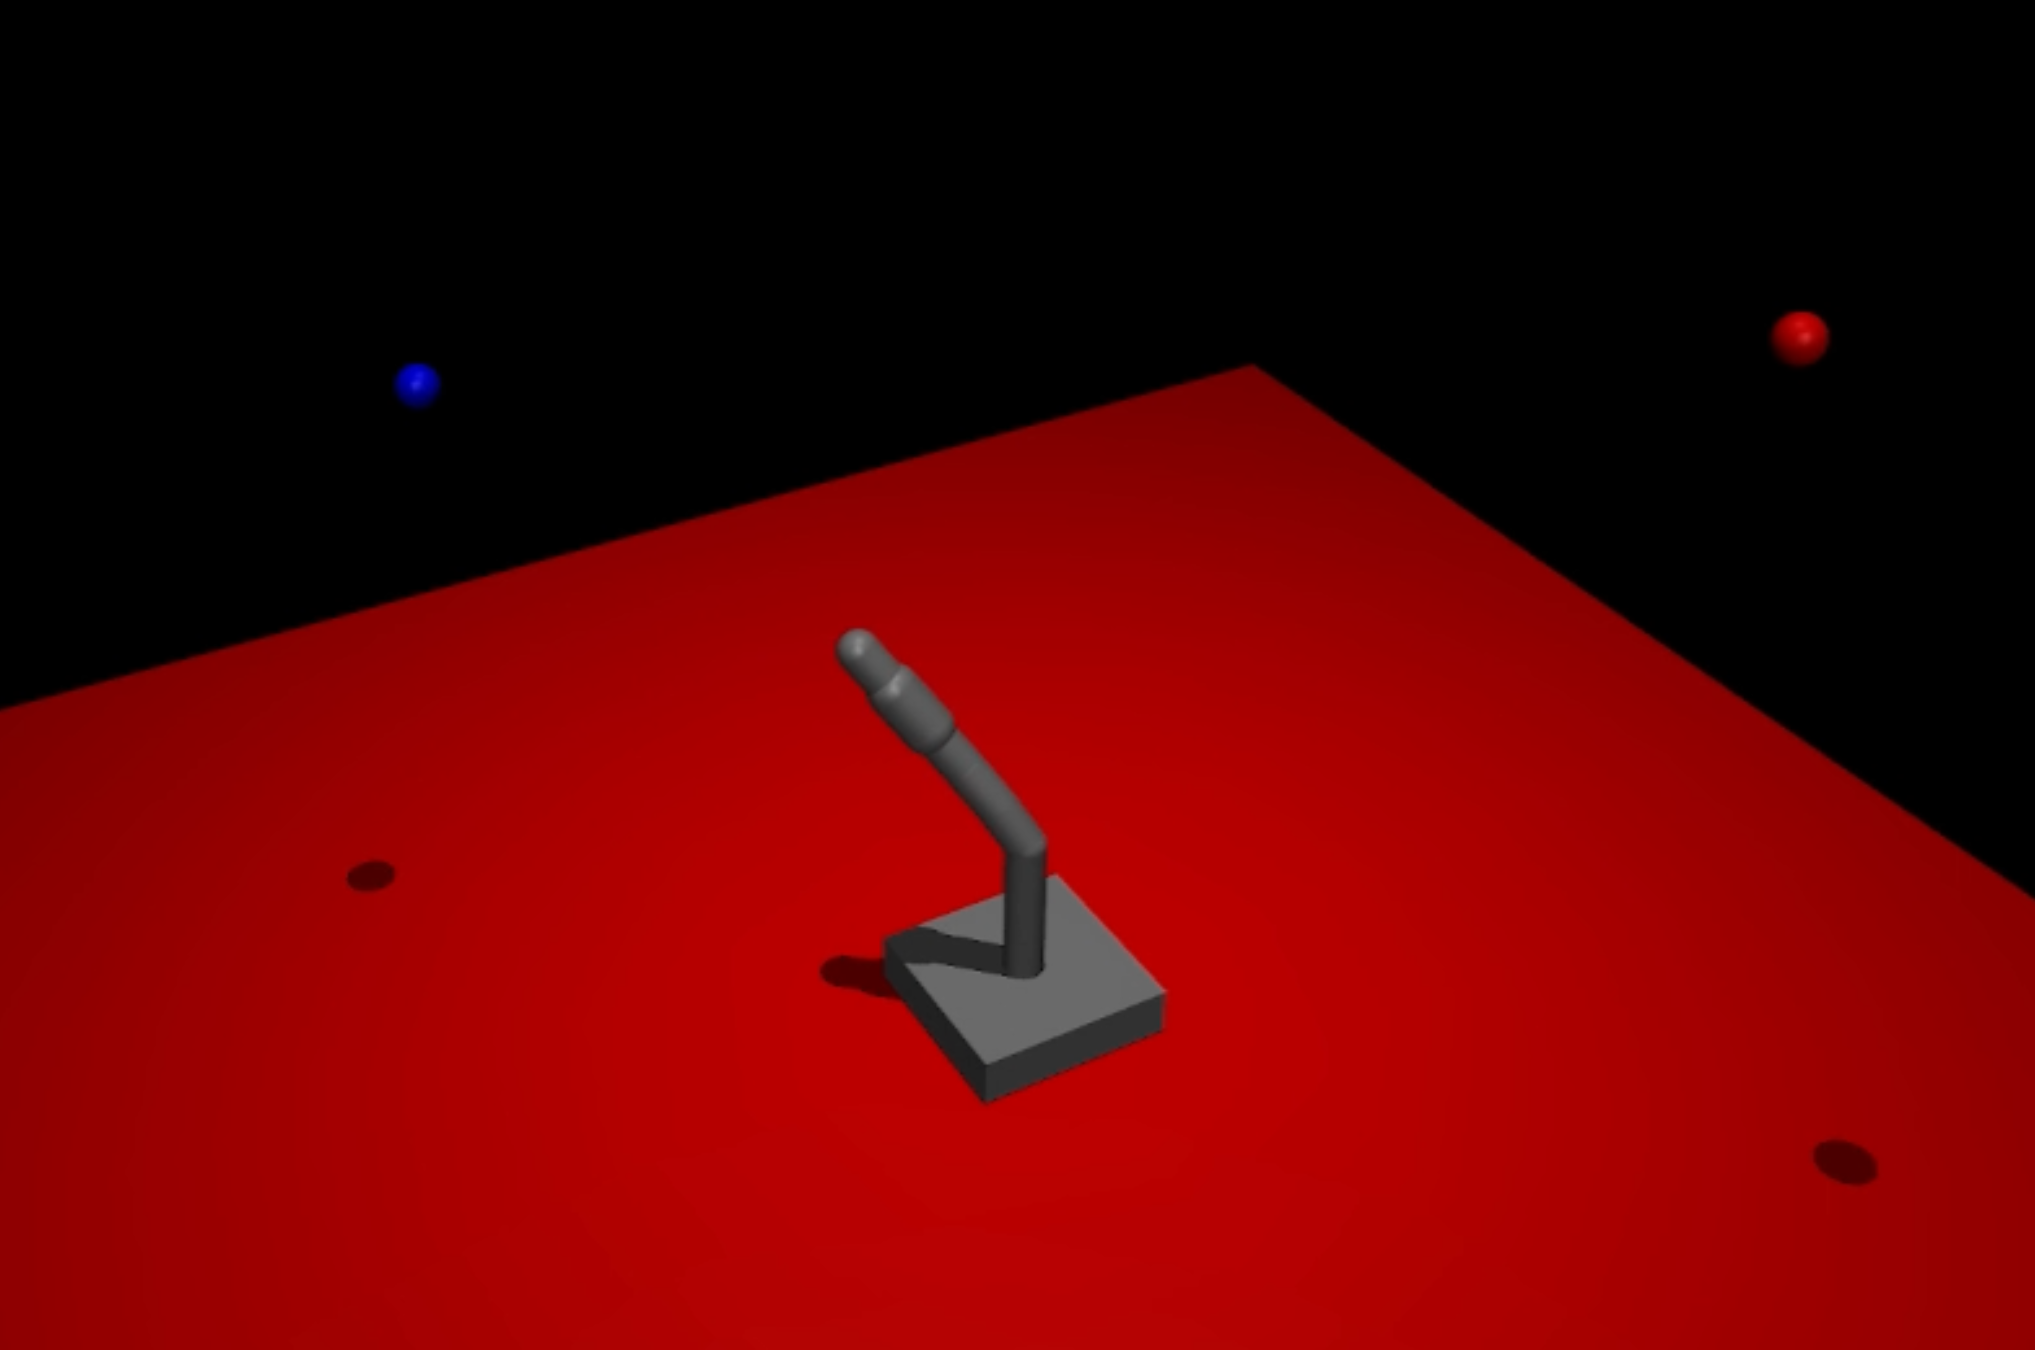
\includegraphics[width=0.9\columnwidth]{firstTask.png}
\caption{Simple Pick and Place Task}
\label{firstTask}
\end{figure}

We started with a simple environment with no obstacles and a simplified reward function (punishment for distance from start and goal points and for path length).
In figure \ref{firstTask} you can see the blue and red dots representing the start and goal points and the first PPO optimized arm that we generated.
Part of the learning and challenge of this method is shaping the reward function and you can see from the image that distance from start and goal was not punished enough resulting in an arm that could not actually reach the objectives.
As you'll see in table \ref{performanceTable} the baseline actually scores higher using the finalized reward function for this reason.

\begin{figure}[H]
\centering

\includegraphics[width=0.9\columnwidth]{shelfTask.png}
\caption{Shelf Task}
\label{shelfTask}
\end{figure}

Then we increased the complexity of the task and the reward function by adding an obstacle and a bonus for manipulability index.
As you can see in figure \ref{shelfTask}, the task now involves a more vertical movement but with an obstacle in the way the agent would have to learn to make an arm that can go around it efficiently.
Unfortunately, the agent learned to go around it too efficiently, exploiting a weakness in the slide design where the slide joints did not have reasonable limits and only consisted of one component so that when they extended there was a physical gap in the arm that could be used to avoid obstacles.
An important learning lesson at this point was that this agent is very good at exploiting weaknesses in the set up so that foundation has to be very strong to build upon.

\begin{figure}[H]
\centering
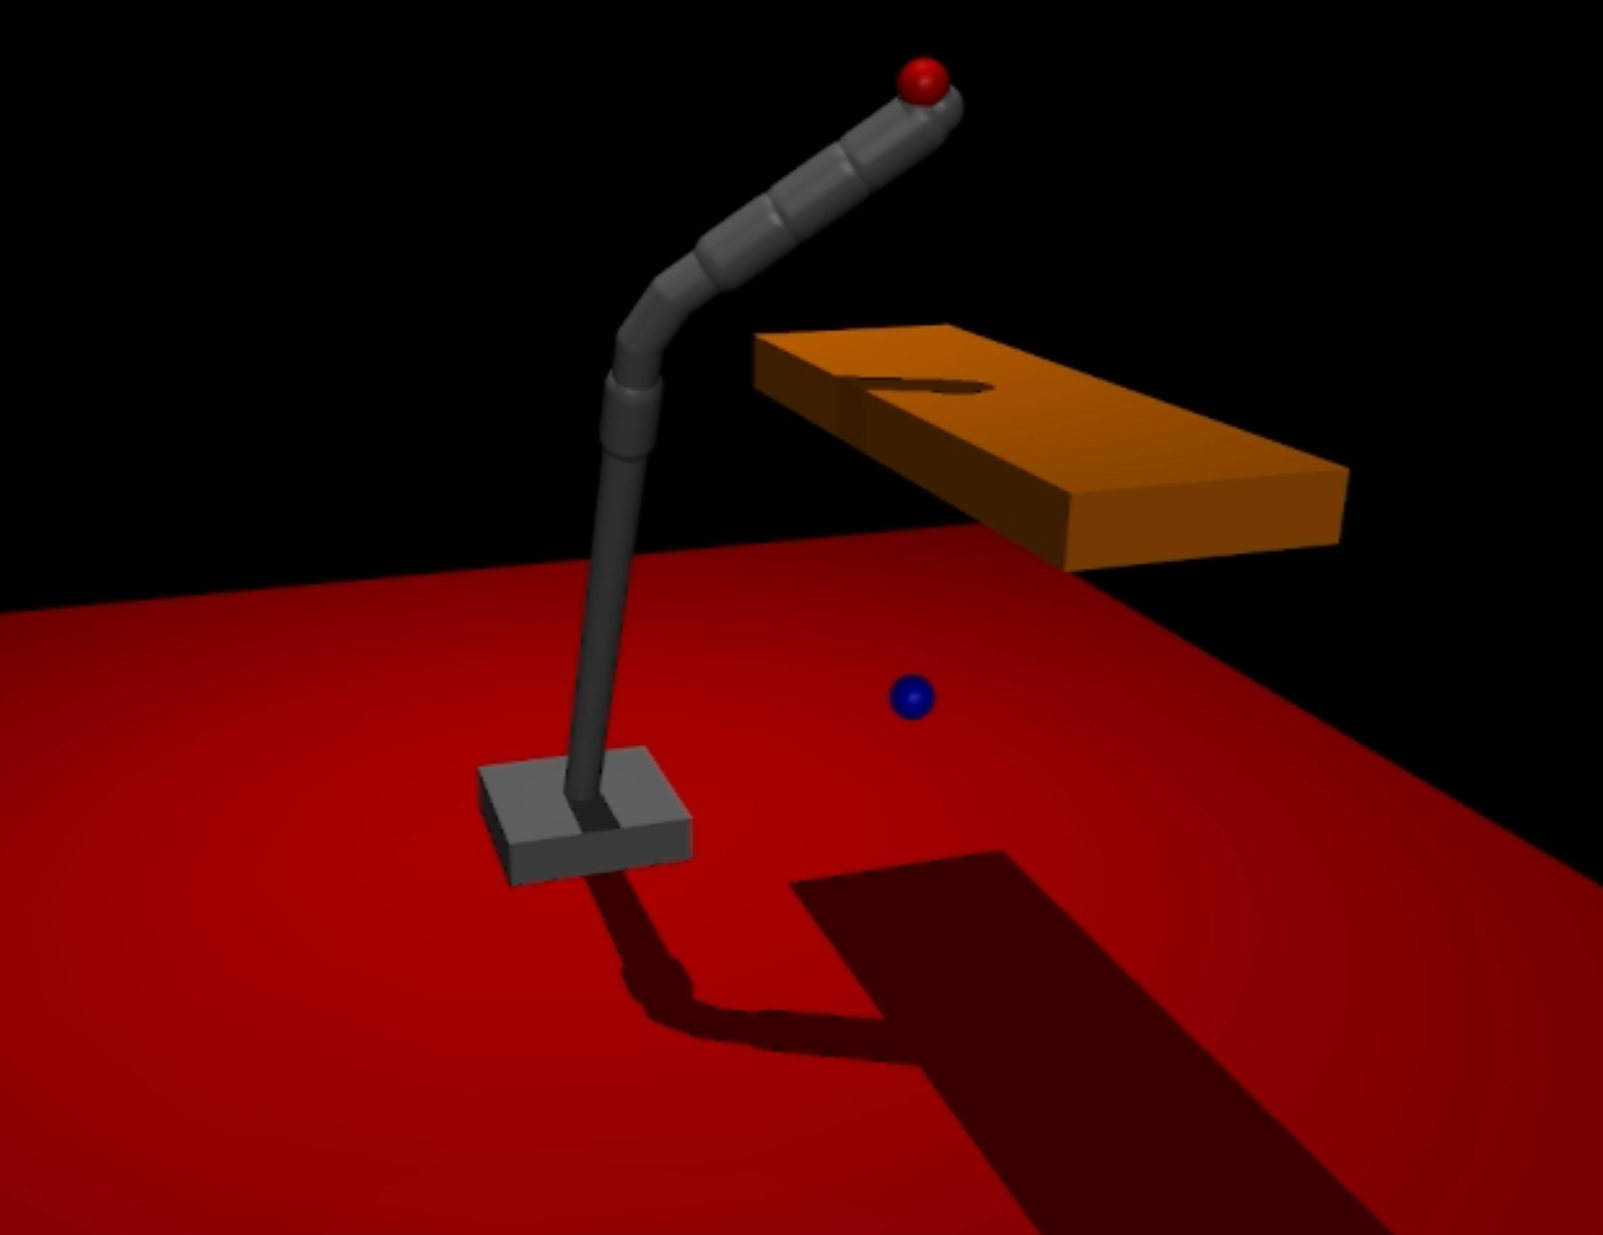
\includegraphics[width=0.9\columnwidth]{shelfFixedSlide.png}
\caption{Shelf Task Two Piece Slide Joints}
\label{shelfFixedSlide}
\end{figure}

In figure \ref{shelfFixedSlide} you can see the fixed slide joint which is made of two pieces of the same length (slightly wider base piece and thinner slide piece) with a joint limit of the link length so that there is never a gap in the arm.

\begin{figure}[H]
\centering
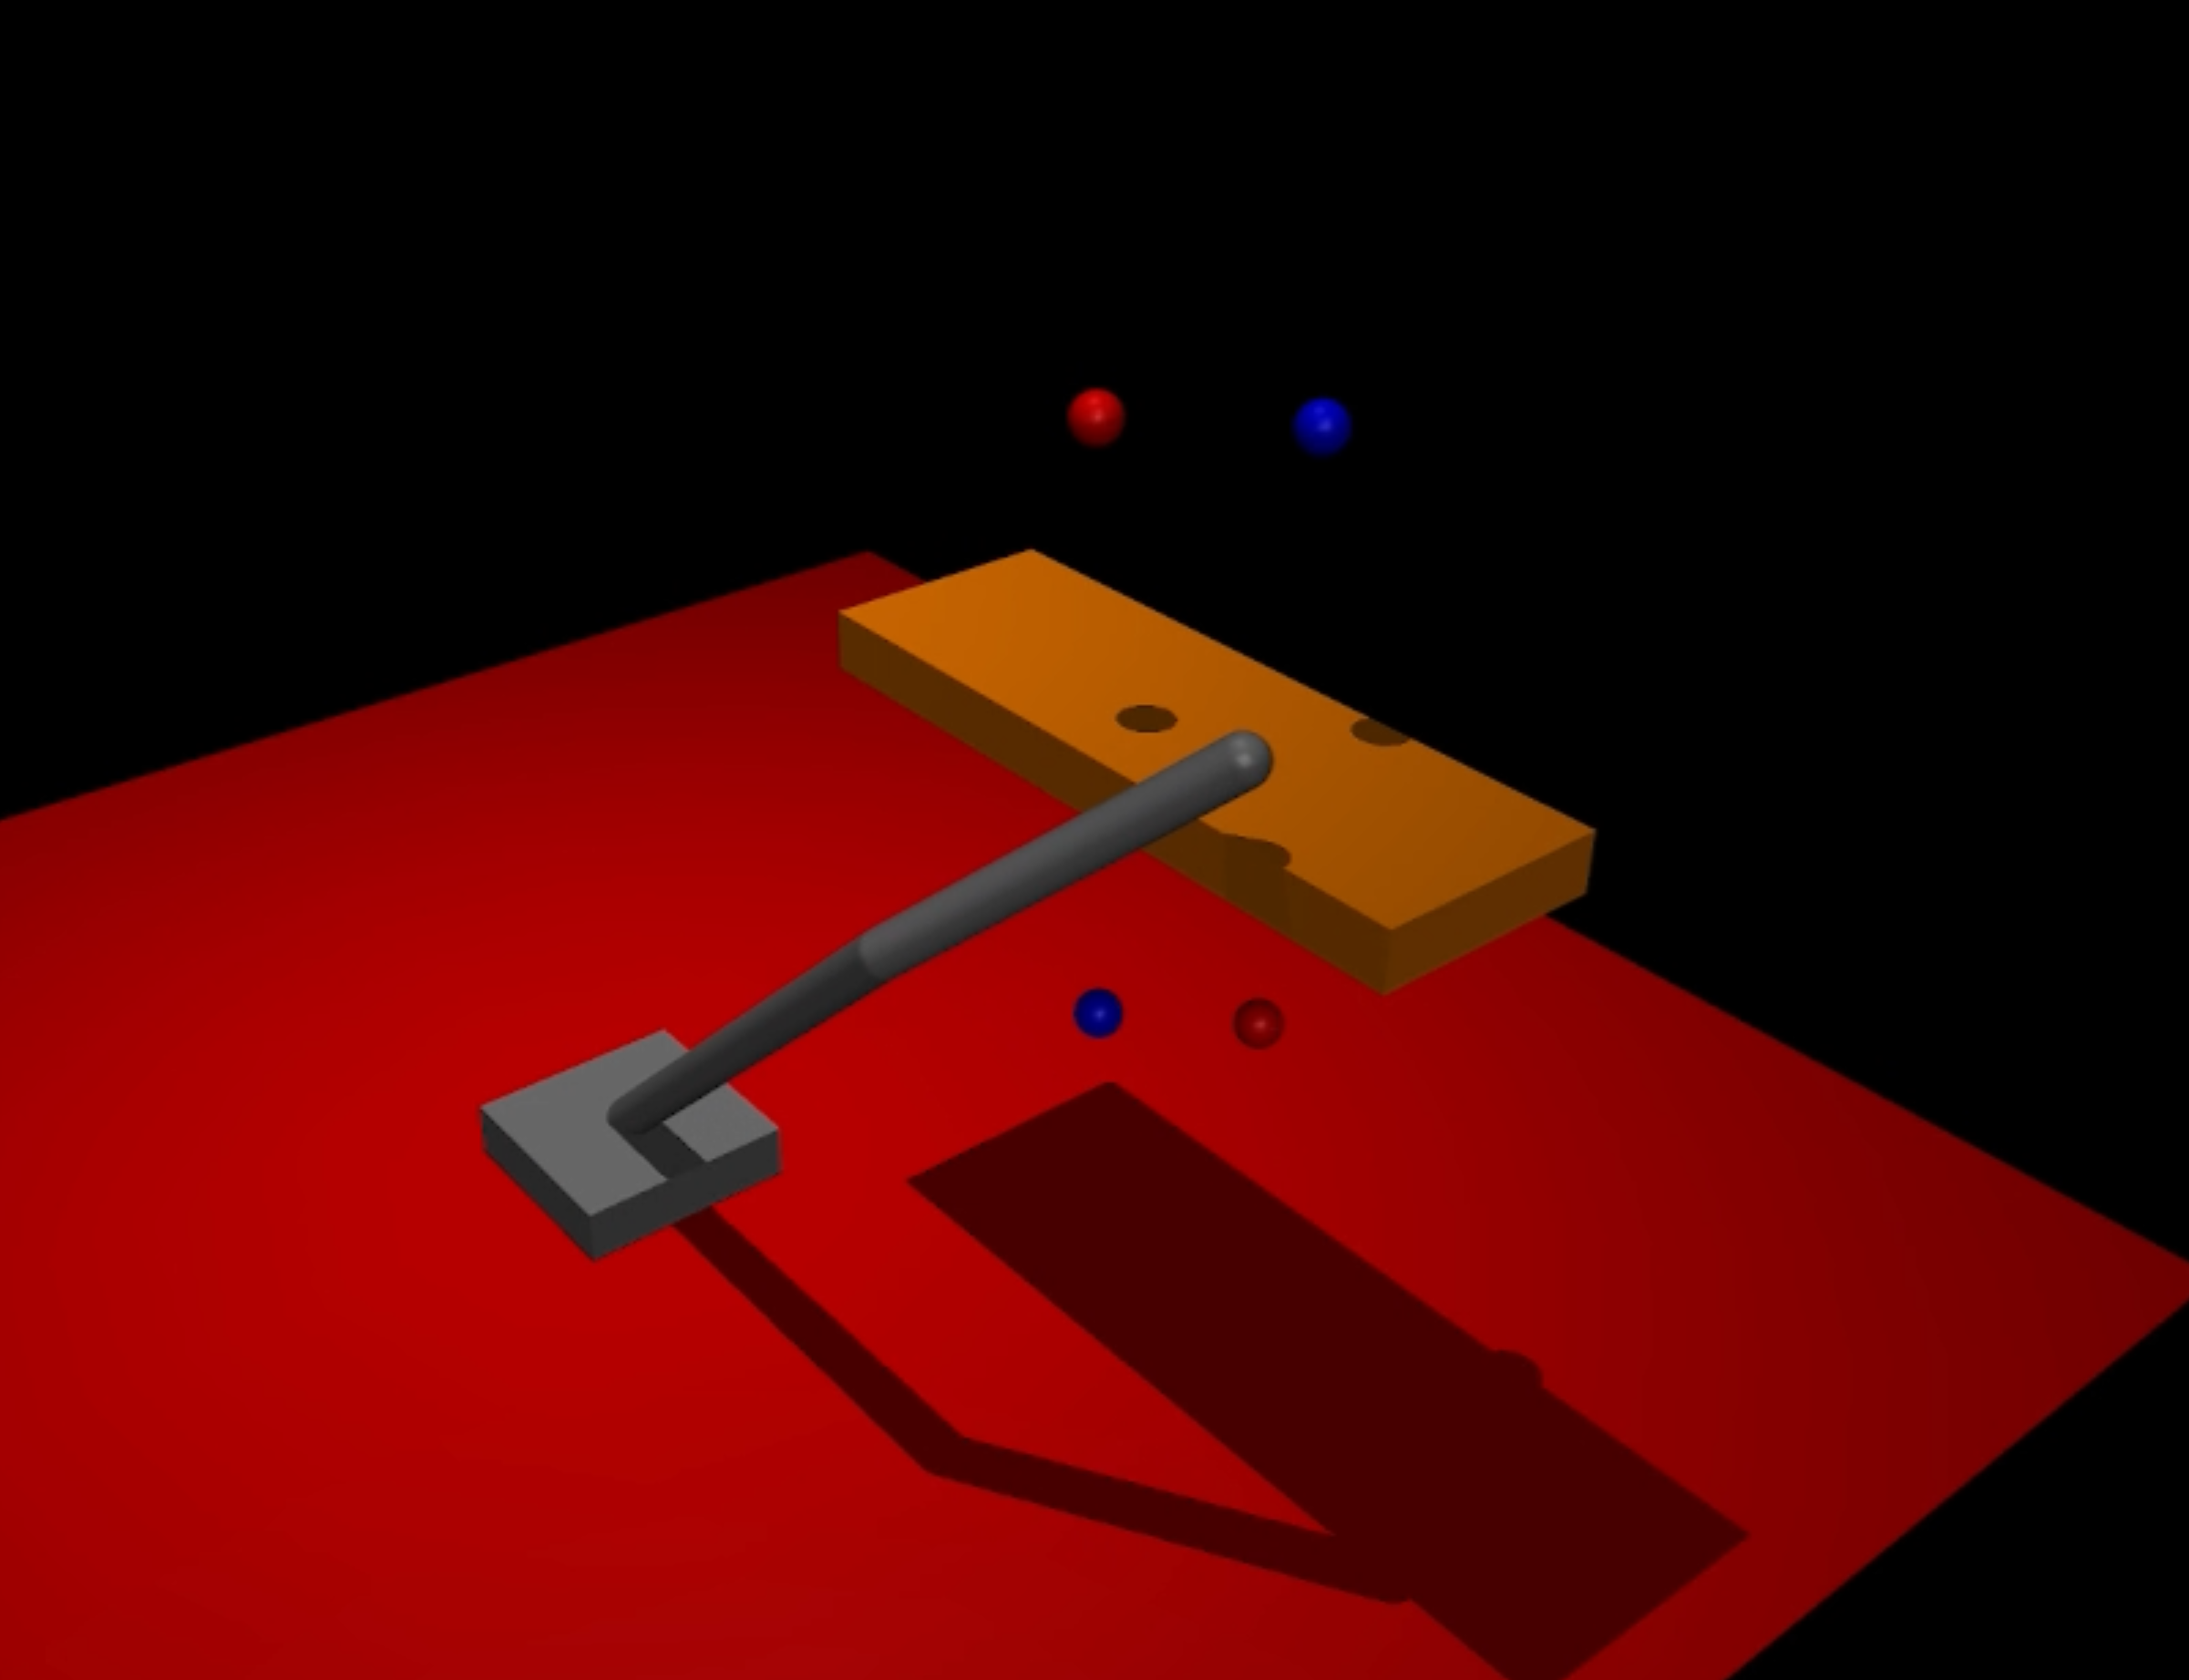
\includegraphics[width=0.9\columnwidth]{shelfMulti.png}
\caption{Shelf with Multiple Tasks}
\label{shelfMulti}
\end{figure}

\begin{figure}[H]
\centering
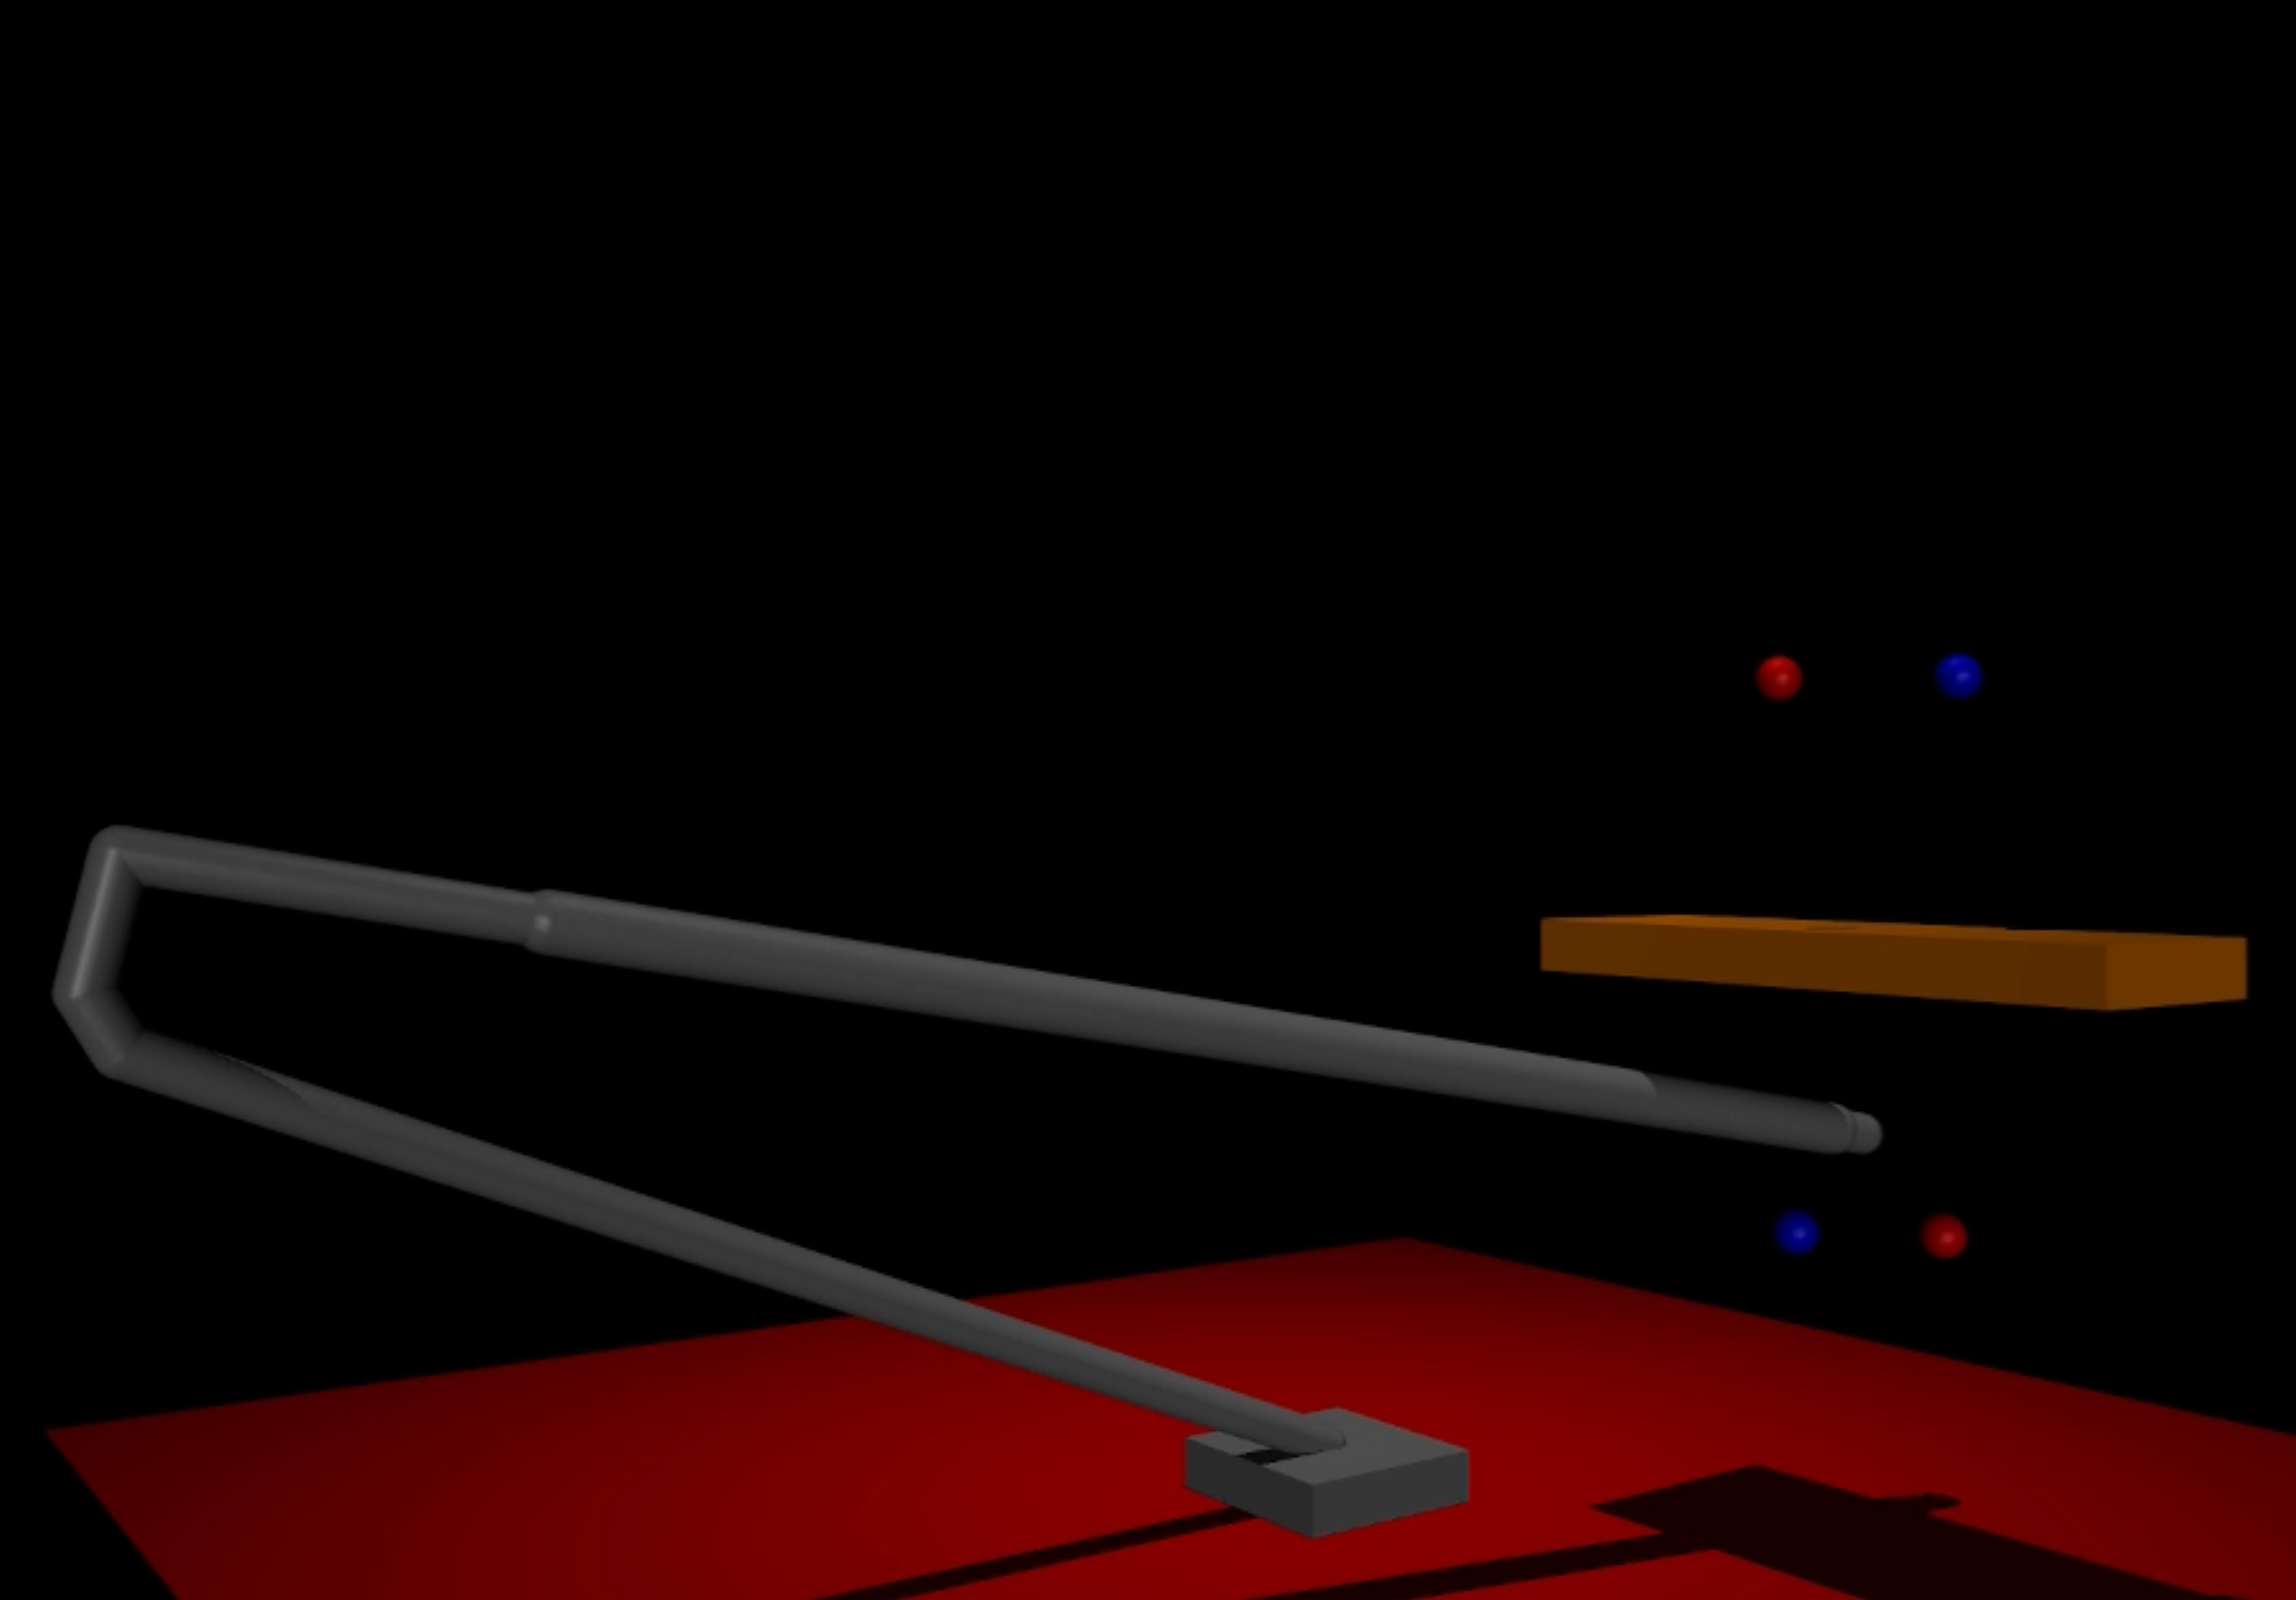
\includegraphics[width=0.9\columnwidth]{shelfMultiHighMan.png}
\caption{Shelf with Multiple Tasks and Higher Manipulability Reward}
\label{shelfMultiHighMan}
\end{figure}

Figures \ref{shelfMulti} and \ref{shelfMultiHighMan} show the experiments in adding tasks and tuning the reward function in the shelf task in an attempt to make arms that are more robust to small variations in the task and environment. An unexpected result of the manipulability index reward term is that slide joints contribute significantly to the manipulability index and so instead of the intended result of more complex, robust arms the result was more slide joints.

\begin{figure}[H]
\centering
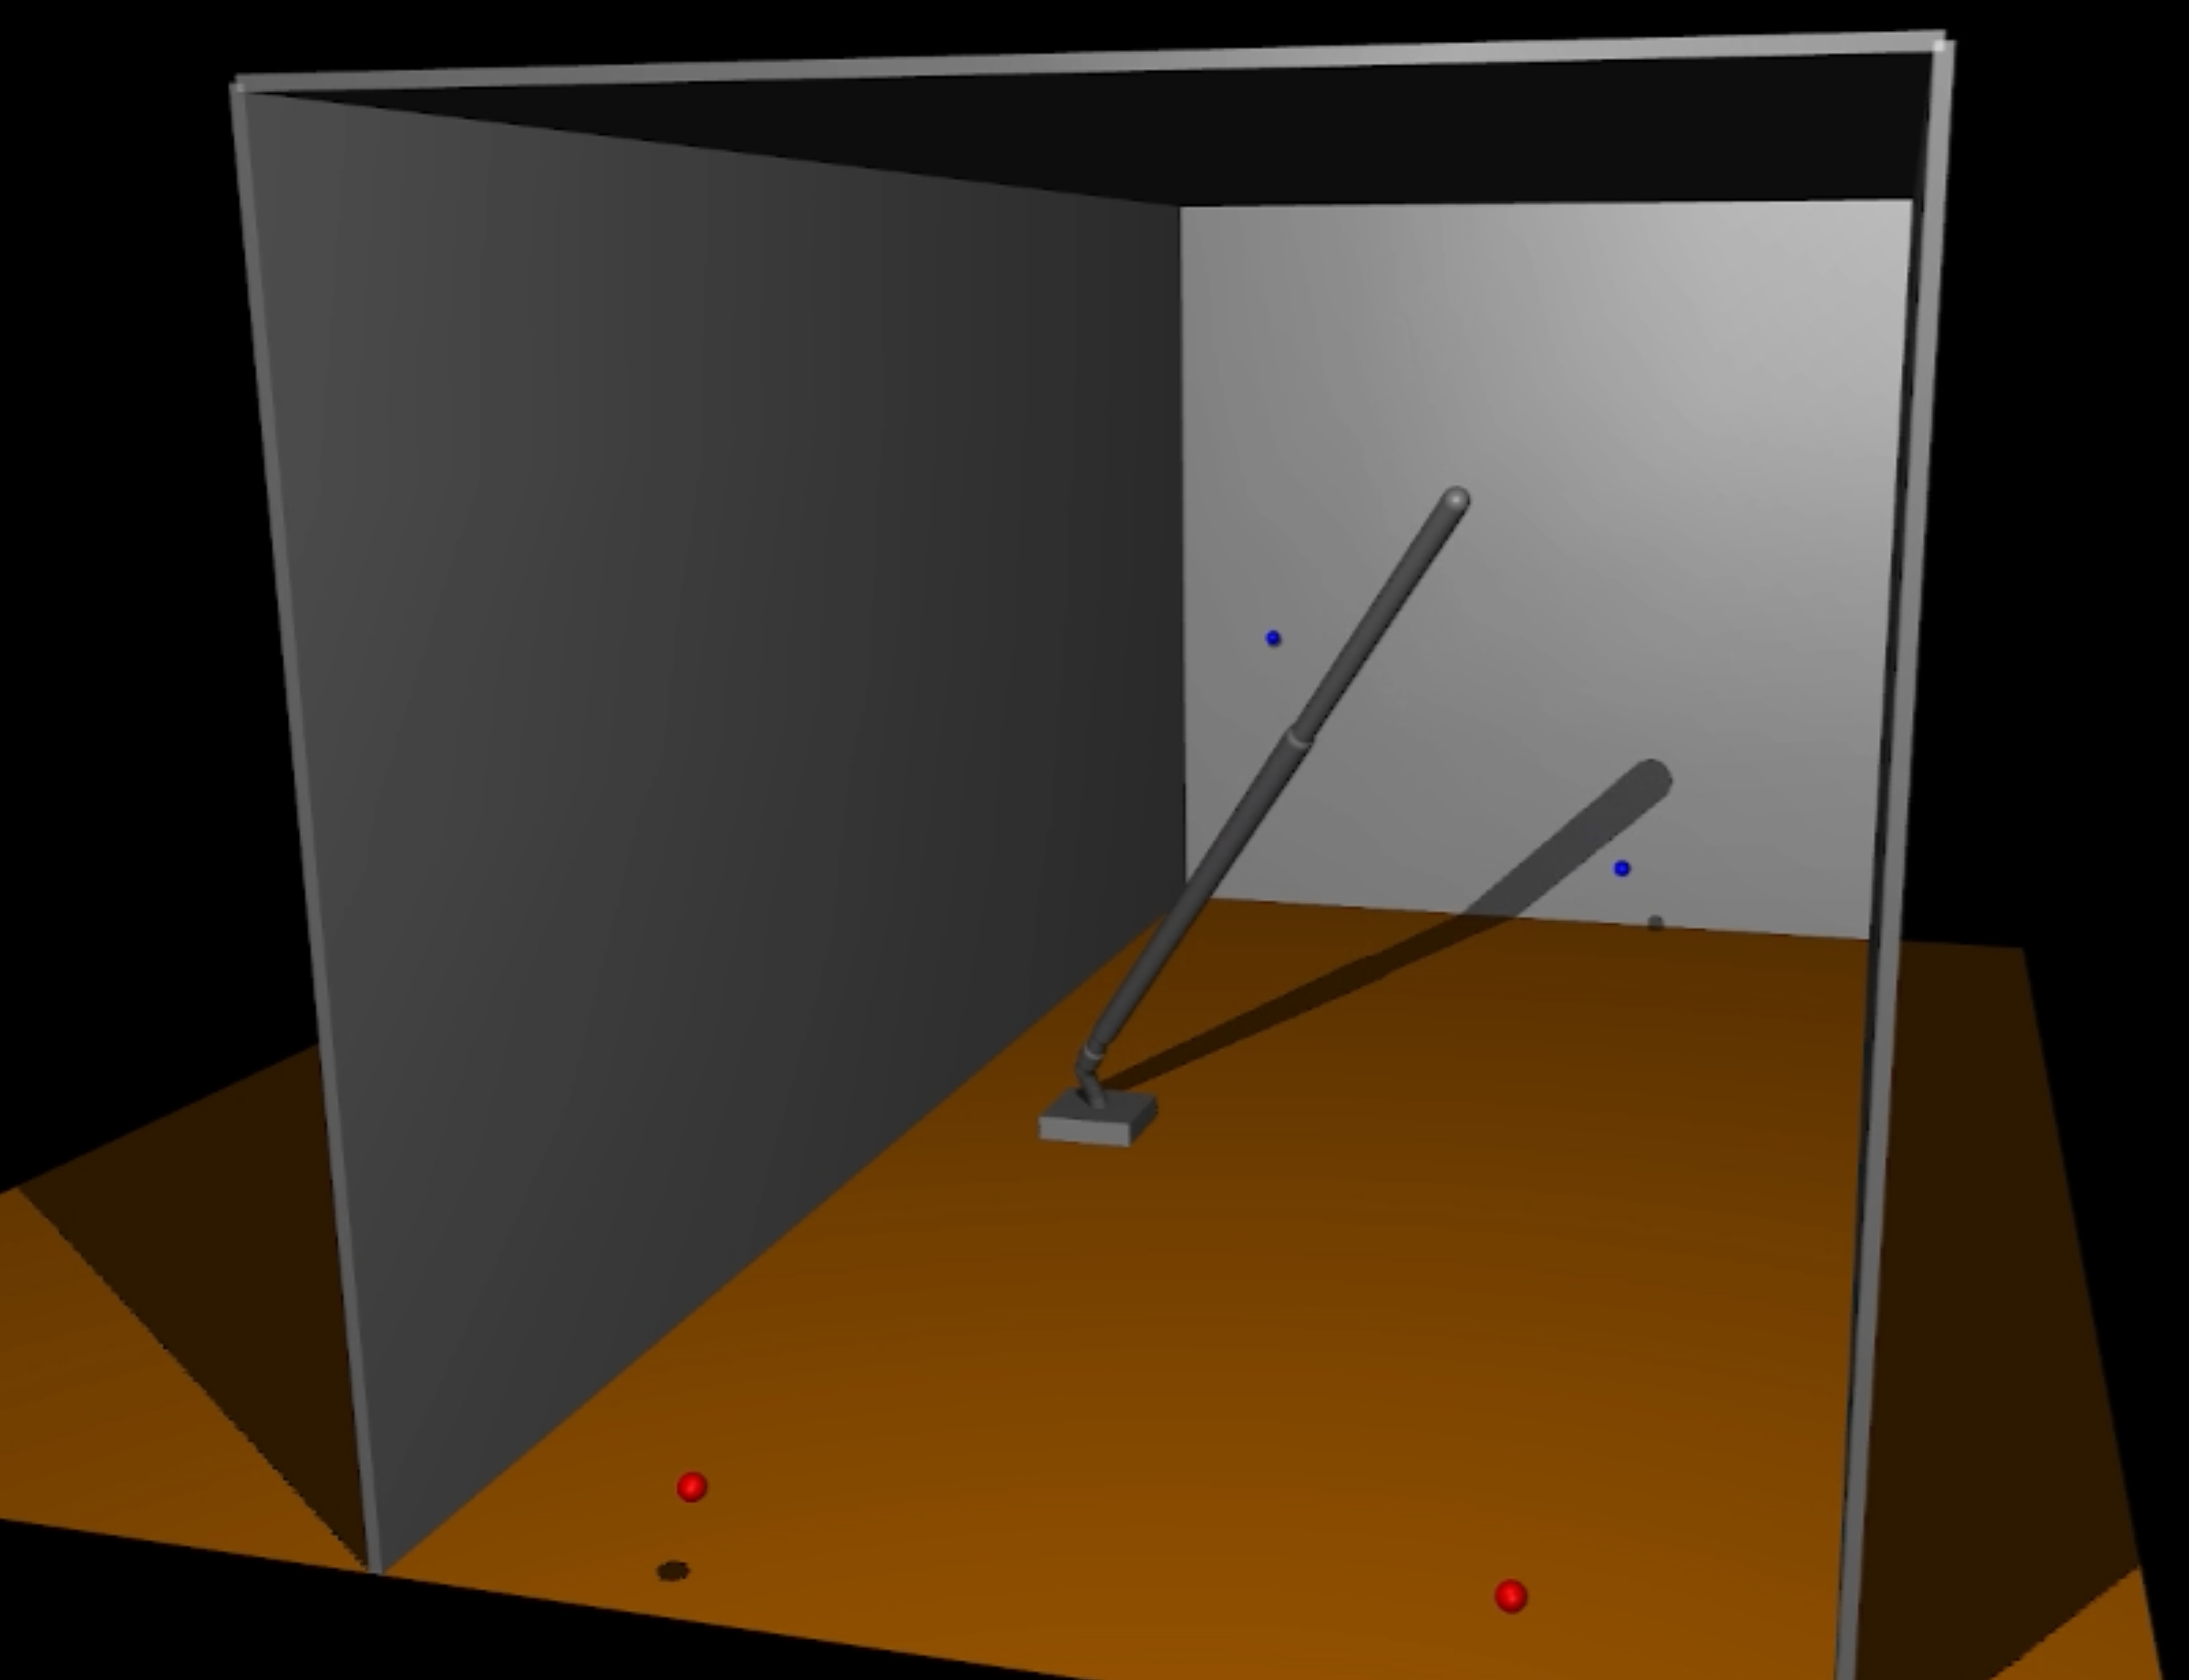
\includegraphics[width=0.9\columnwidth]{containerTask.png}
\caption{Container Task (Constrained Environment)}
\label{containerTask}
\end{figure}

For the constrained environment task, we surrounded the arm with wall and ceiling obstacles and put the start and goal points at either end as if the arm were unloading a truck.
Figure \ref{containerTask} shows the environment and the resulting, optimized arm.

\begin{figure}[H]
\centering
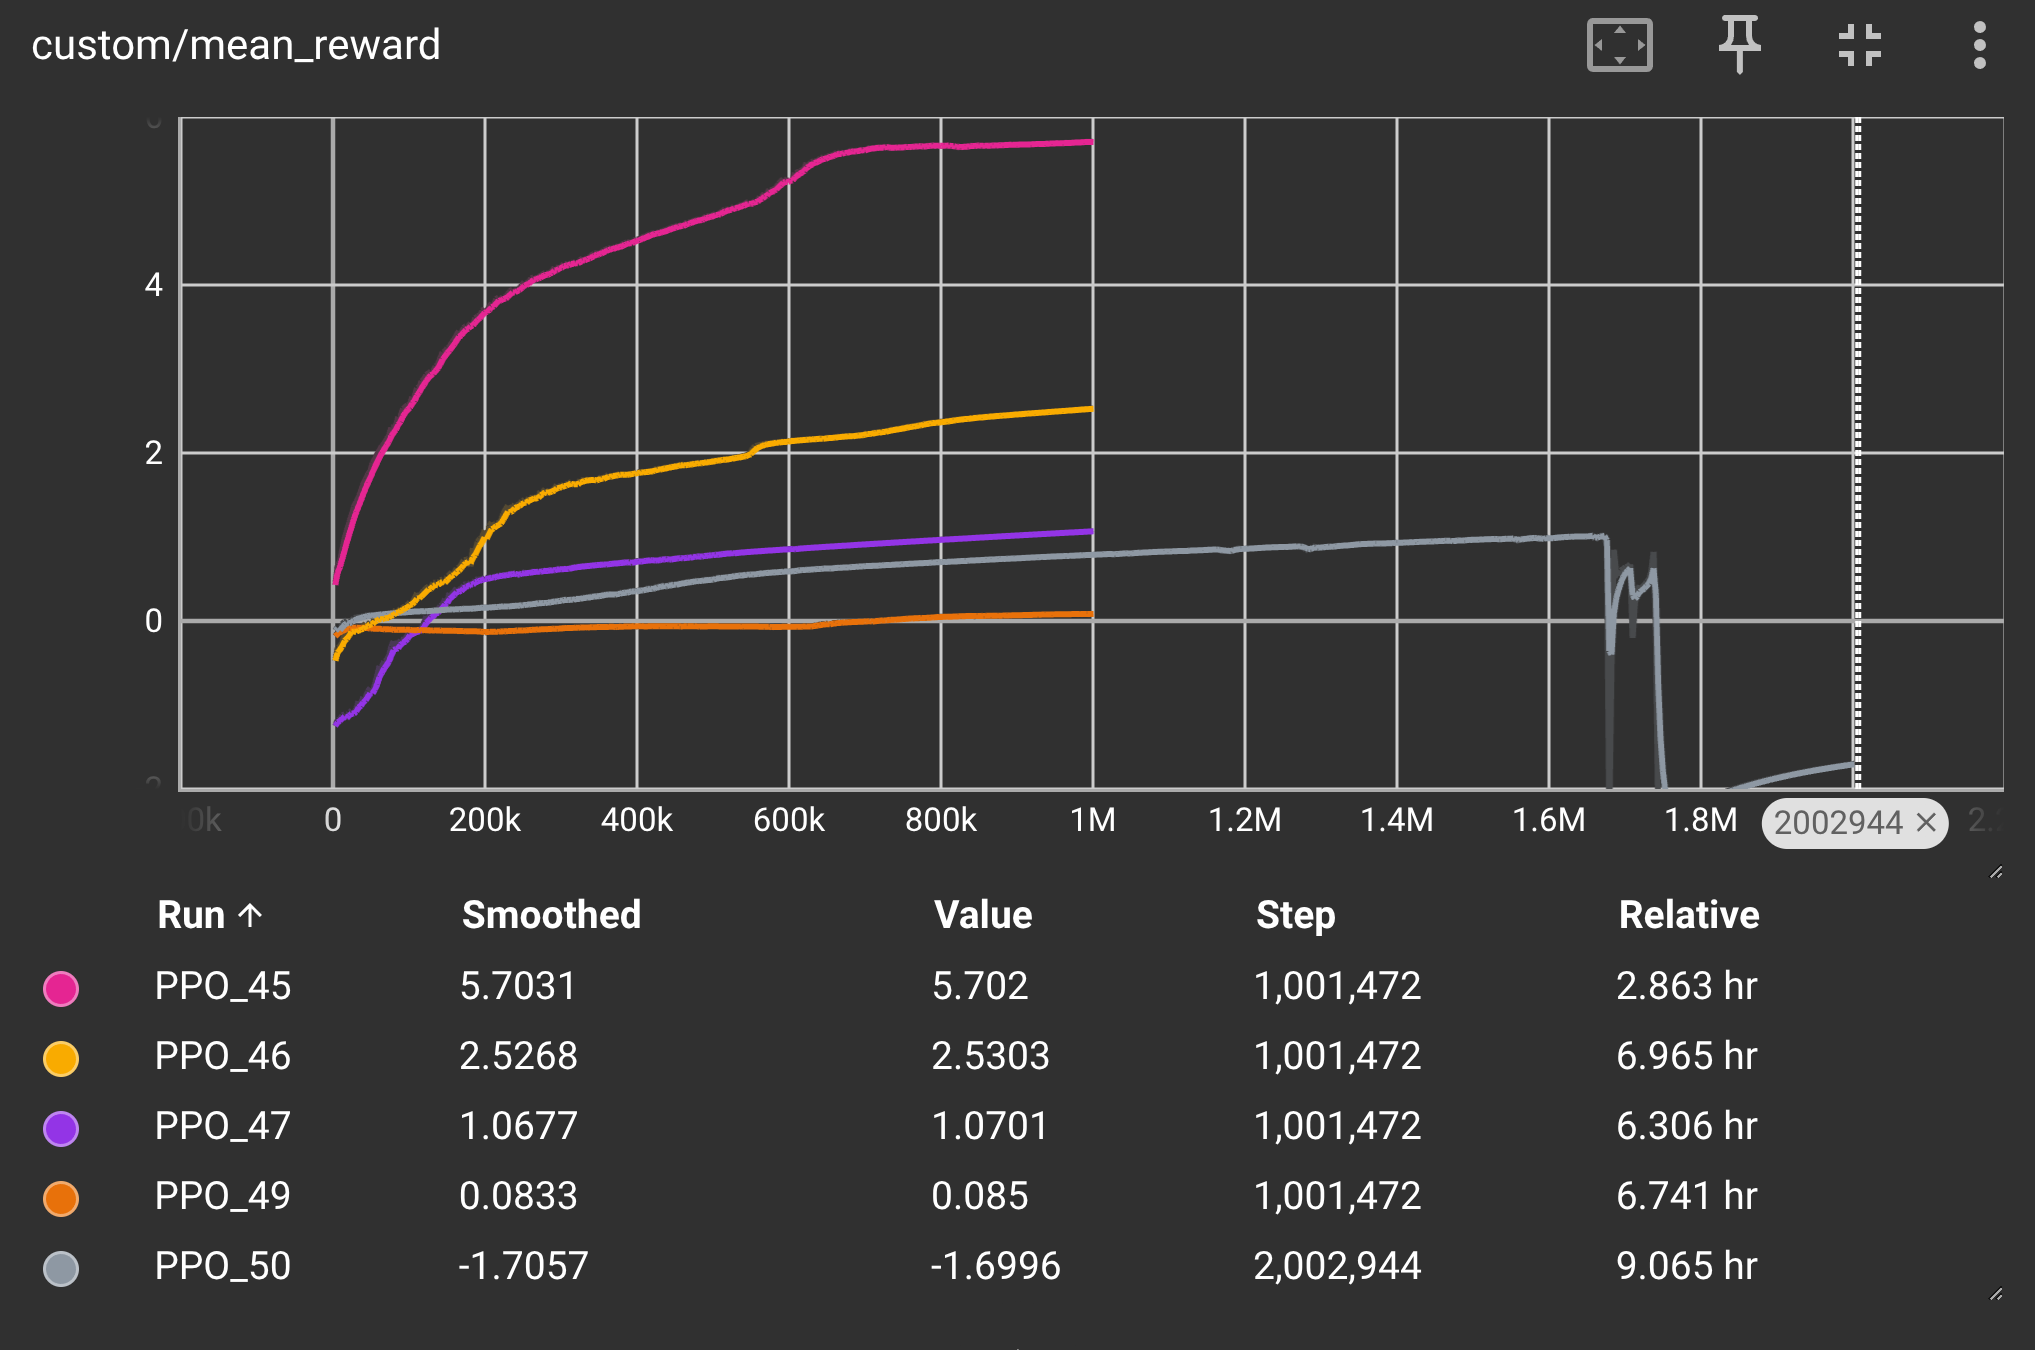
\includegraphics[width=0.9\columnwidth]{rewardCurve.png}
\caption{Rewards per Episode Plot}
\label{rewardCurve}
\end{figure}

Figure \ref{rewardCurve} shows the averaged, normalized rewards during the training of the various tasks. PPO\_45 corresponds to the initial shelf task shown in figure \ref{shelfTask}, PPO\_46 corresponds to the first multi shelf task (figure \ref{shelfMulti}), PPO\_47 to the second one with a higher manipulability score (figure \ref{shelfMultiHighMan}), PPO\_49 is the container task (figure \ref{containerTask}), and PPO\_50 shows the curve for another failed contrained task (figure \ref{wallTask}) that will be discussed in the Conclusion section.

\begin{table}[H]
\centering
\small % Use small font to help fit
\caption{Performance Metrics for Panda and Optimized Arm Across Tasks}
\label{tab:performance-metrics}
\resizebox{\columnwidth}{!}{
\begin{tabular}{l|l|c|c|c|c|c|c}
\toprule
Task & Arm & Score & Success & Acc. Penalty & Manip. Bonus & Link Penalty & Path Penalty \\
\midrule
Simple & Panda & 86.7 & 100 & -0.8 & 0.3 & -12.5 & -0.3 \\
\midrule
       & Optimized & -48.86 & 100 & -137 & 0.65 & -12.5 & -0.01 \\
\midrule
Shelf & Panda & 85 & 100 & -0.08 & 0.49 & -12.5 & -0.2 \\
\midrule
      & Optimized & 117 & 100 & -0.15 & 30.37 & -12.5 & -0.09 \\
\midrule
Container & Panda & 56.7 & 100 & -31.2 & 1.2 & -12.5 & -0.8 \\
\midrule
          & Optimized & 115 & 100 & -0.07 & 57 & -12.5 & -0.5 \\
\bottomrule
\end{tabular}
}
\label{performanceTable}
\end{table}

Table \ref{performanceTable} shows the results of evaluating the task optimized arms versus a standard Franka Emika Panda baseline. Figure \ref{panda} shows the baseline morphology that was used to compare against. The basic joint types and dimensions of a standard Franka Emika Panda were used.

\begin{figure}[H]
\centering
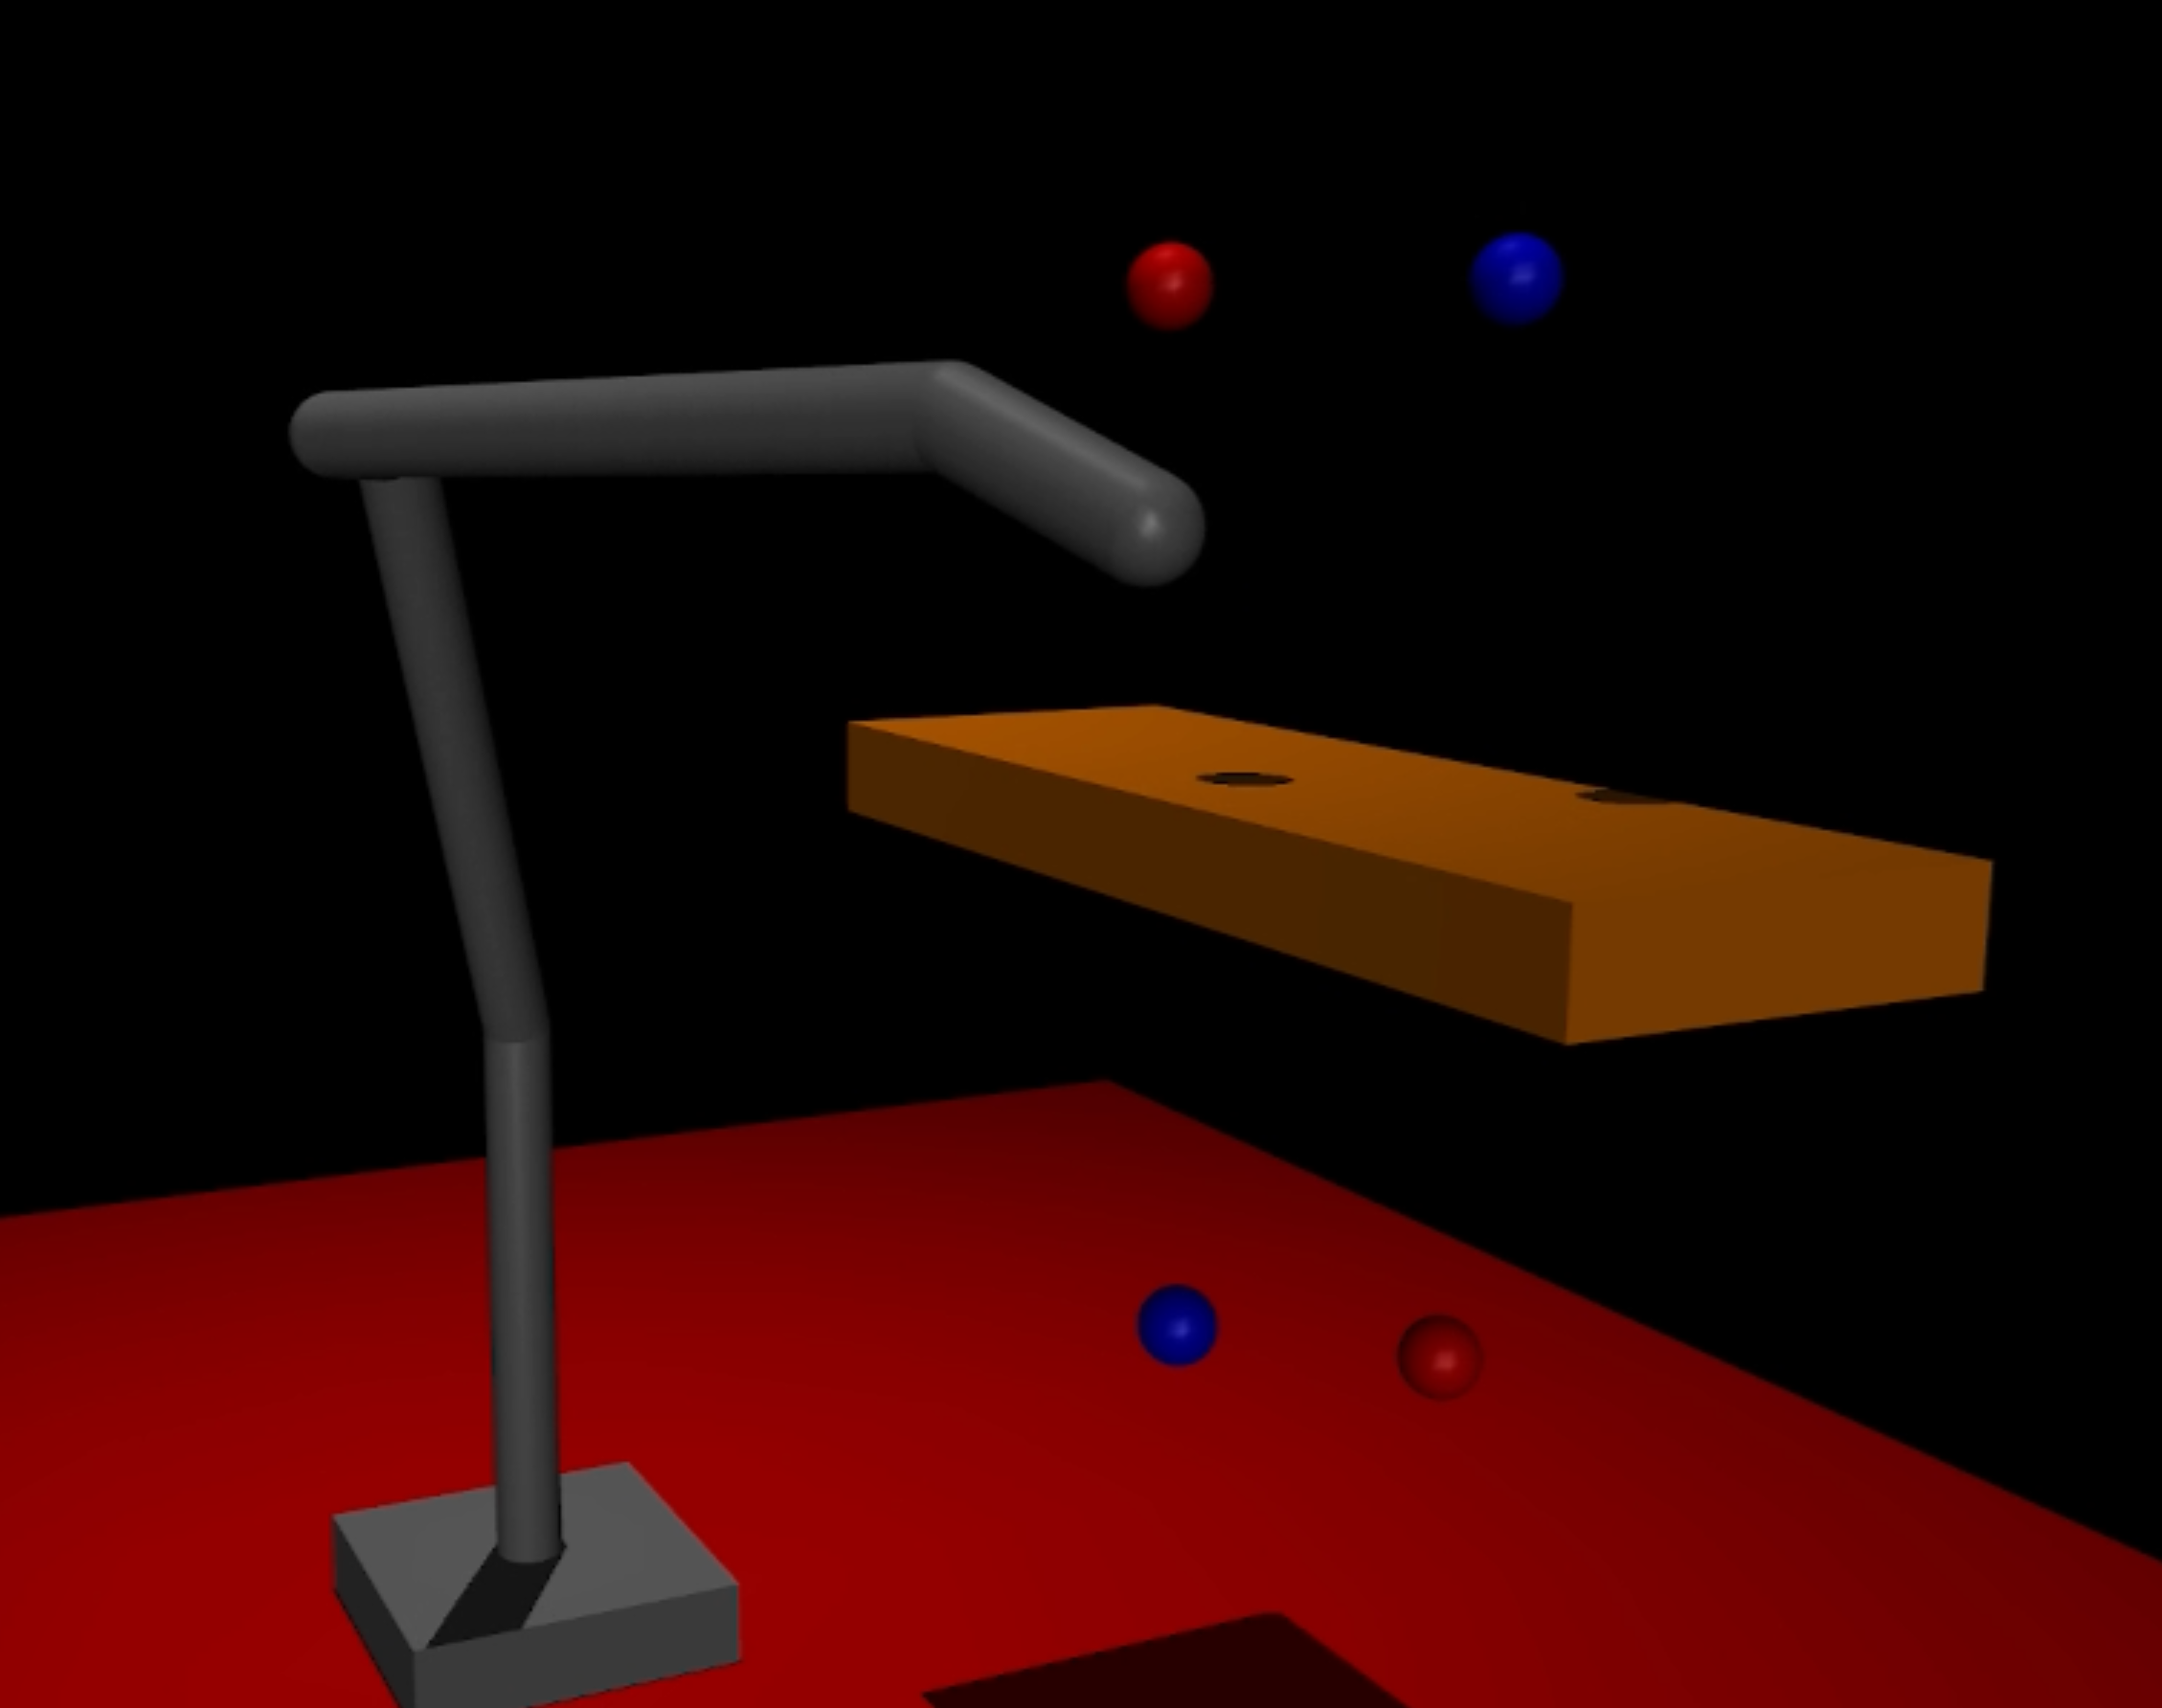
\includegraphics[width=0.9\columnwidth]{panda.png}
\caption{Franka Emika Panda Baseline}
\label{panda}
\end{figure}

The performance was better for the optimized arms than the baseline in each task except the simple task which was trained on an early iteration of the reward function. The optimized arms show shorter path lengths and higher manipulability with the accuracy results being mixed.

\section{Conclusion}

The problem in using PPO to design a robot arm morphology is very much in the definition of the environment and the shaping of the reward. The optimized arms perform better in terms of the reward function they were optimized around. The arms generated and tested here got a bonus in manipulability measure by learning to use slide joints. However, using slide joints might not be meaningful in practice because the very directional manipulability that they add might not add anything practical.

Another issue with the optimized arms can be seen most notably in figure \ref{containerTask} where the arm has mostly small hinge joints at the base and then long slide joints that allow it to reach the start and goals and the path that it takes is very long tall arches as it goes from the start, up over its base, and back down the other side to the goals. This type of movement would require a lot of mechanical power in reality to hold the weight of the fully extended arm out against gravity using the motors in the small base joints.

This realization led to the final task environment and reward function that were not fully implemented in time for this paper. An energy cost term was added to the reward function and was calculated using MuJoCo's built-in inverse dynamics to get the mechanical power of the trajectories ($torque \cdot velocity$) and subtract that from the reward to punish higher energy using morphologies. Then we set up one last environment where the arm was mounted sideways on a wall and had start and goal positions from the floor onto a shelf as you can see in figure \ref{wallTask}.

\begin{figure}[H]
\centering
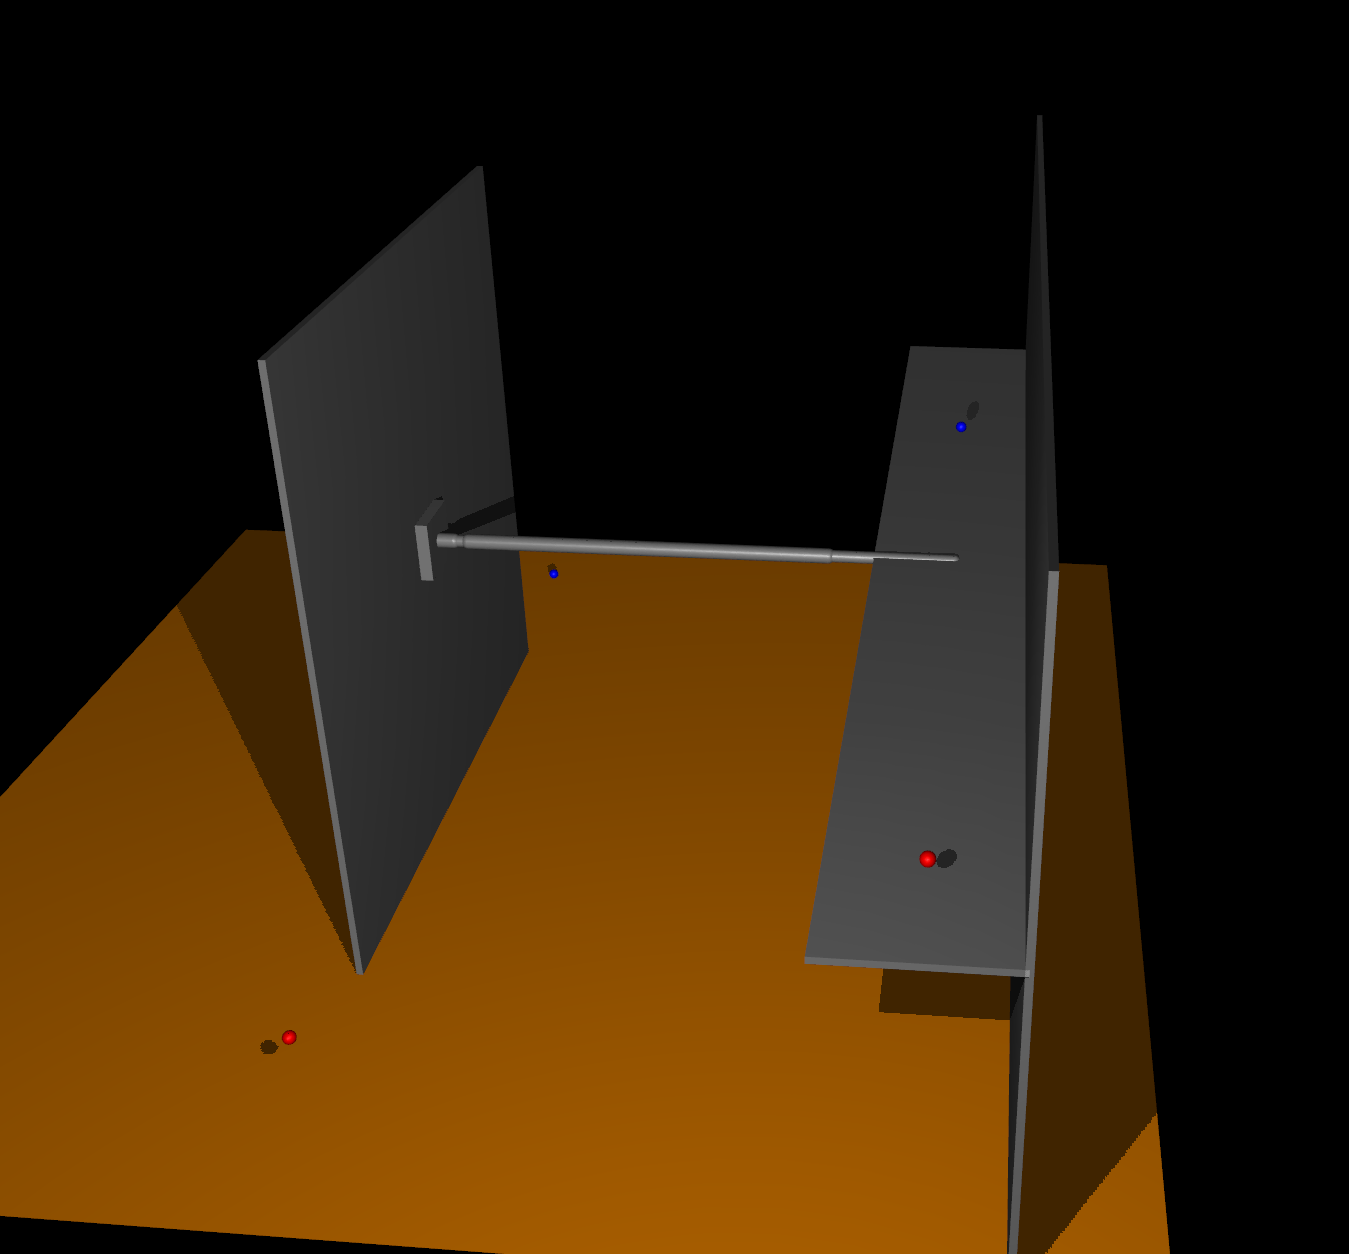
\includegraphics[width=0.9\columnwidth]{wallTask.png}
\caption{Wall Mounted Task with Energy Cost Reward}
\label{wallTask}
\end{figure}

If you look in figure \ref{rewardCurve} you can see the reward curve for this task (PPO\_50) was quite low and hit some drop offs around 1.7 million episodes.
Our hypothesis is that this task is a bit trickier than previous tasks and a lot more morphologies would fail because of the difficult start and goal placements and all of the obstacles and the models exploration led it into some unfortunate local minima as it went on.

Our hope for the future is to continue refining the environment and reward function.
We want to remove the manipulability index and try other measures for robustness and complexity.
Something I talked about in the proposal but did not implement here was introducing Guassian noise into the start and goal positions to provide some more robustness in the designs.
We would also like to successfully implement the energy cost term and so might start that on an easier environment in the future.

\section{Contributions and Roles}
Steve Gillet is responsible for the RL implementation and initial simulation setup including PPO and baseline setups, reward design, ablations, and primary experiments on optimization and efficiency
He owns the learning curves and rewards tables and RL-specific metrics in evaluations.

Jay Vakil handles the simulation environment including multi model generation in MuJoCo, REAL RL implementation, and any other evaluations.
He owns the codebase maintenance and any other evaluation graphics used.

\bibliographystyle{IEEEtran}
\bibliography{references}

\end{document}